% Copyright (C) 2013 Columbia University in the City of New York and others.
%
% Please see the AUTHORS file in the main source directory for a full list
% of contributors.
%
% This file is part of TerraFERMA.
%
% TerraFERMA is free software: you can redistribute it and/or modify
% it under the terms of the GNU Lesser General Public License as published by
% the Free Software Foundation, either version 3 of the License, or
% (at your option) any later version.
%
% TerraFERMA is distributed in the hope that it will be useful,
% but WITHOUT ANY WARRANTY; without even the implied warranty of
% MERCHANTABILITY or FITNESS FOR A PARTICULAR PURPOSE. See the
% GNU Lesser General Public License for more details.
%
% You should have received a copy of the GNU Lesser General Public License
% along with TerraFERMA. If not, see <http://www.gnu.org/licenses/>.


\chapter{Magmatic Solitary Wave Benchmarks: \citeauthor{simpson_solitary_2011}} \label{sec:simpson} 

Solution of magmatic solitary waves in 2 and 3D (see Figure
\ref{fig:1dto3dwaves}) are compared to spectrally accurate sinc-collocation solutions given in \cite{simpson_solitary_2011}.  These problems solve a completely different set of coupled equations from thermal convection for porosity $\phi$ and ``compaction pressure'' $\mathcal{P}$ \begin{equation}
  \label{eq:15}
  \ppt{\phi} + \vec{v}\cdot\grad\phi =
  \left(\frac{h}{\delta}\right)^{2} \phi^{m}\mathcal{P}
\end{equation}
\begin{equation}
  \label{eq:16}
  -\div\phi^n\grad\mathcal{P} + \left(\frac{h}{\delta}\right)^{2} \phi^{m}\mathcal{P}=\div\phi^n\vec{k}
\end{equation}
(see Figure \ref{fig:simpson_benchmarks}).  These benchmarks are
particularly nice in that they are a fully non-linear solution that
propagates at constant speed $c$ (which depends on wave amplitude)
without changing shape. Any errors in shape or propagation velocity
can be directly attributed to numerical error.  In particular, in a
moving frame with velocity $\vec{v}= (0,-c)$, the waves should appear to
stand still.

These benchmarks are also a good test of advanced advection schemes
for hyperbolic problems and we currently have benchmarks for standard
CG advection without stabilization and semi-Lagrangian advection
schemes.  Figure \ref{fig:simpson_benchmarks} shows errors in shape
and velocity as a function of
mesh and time step refinement for a 2D wave
propagating at speed $c=5$ with permeability exponent $n=3$ and
porosity independent bulk viscosity $m=0$ using a semi-Lagrangian
advection scheme.  Tables \ref{tab:simpson2d}--\ref{tab:simpson3d}
show results for additional 2 and 3D waves. For each table $N$ is the number of square cells in each direction (with right/left diagonals for division into triangles), $c\Delta t/\delta$ is the number of compaction lengths (at the background porosity) that  a solitary wave travels in one time-step,
\begin{displaymath}
  ||e_{\phi}||=\min_\lambda\frac{\sqrt{\int_\Omega(\phi_{exact} - \phi_{h}(\vec{x} - \vec\lambda))^{2}\,dx}}{\sqrt{\int_\Omega(\phi_{exact})^{2}\,dx}}
\end{displaymath}
is the L2 norm of the relative shape error for the numerical wave $\phi_h$ that is translated by phase error $\vec{\lambda}$ to minimize the misfit between the numerical solution and the exact solitary wave \citep[see][for details of error analysis]{simpson_solitary_2011}.  $e_{c} =  1 - c/c_{exact}$ is the relative velocity error.

\begin{figure}[htb]
  \centering
  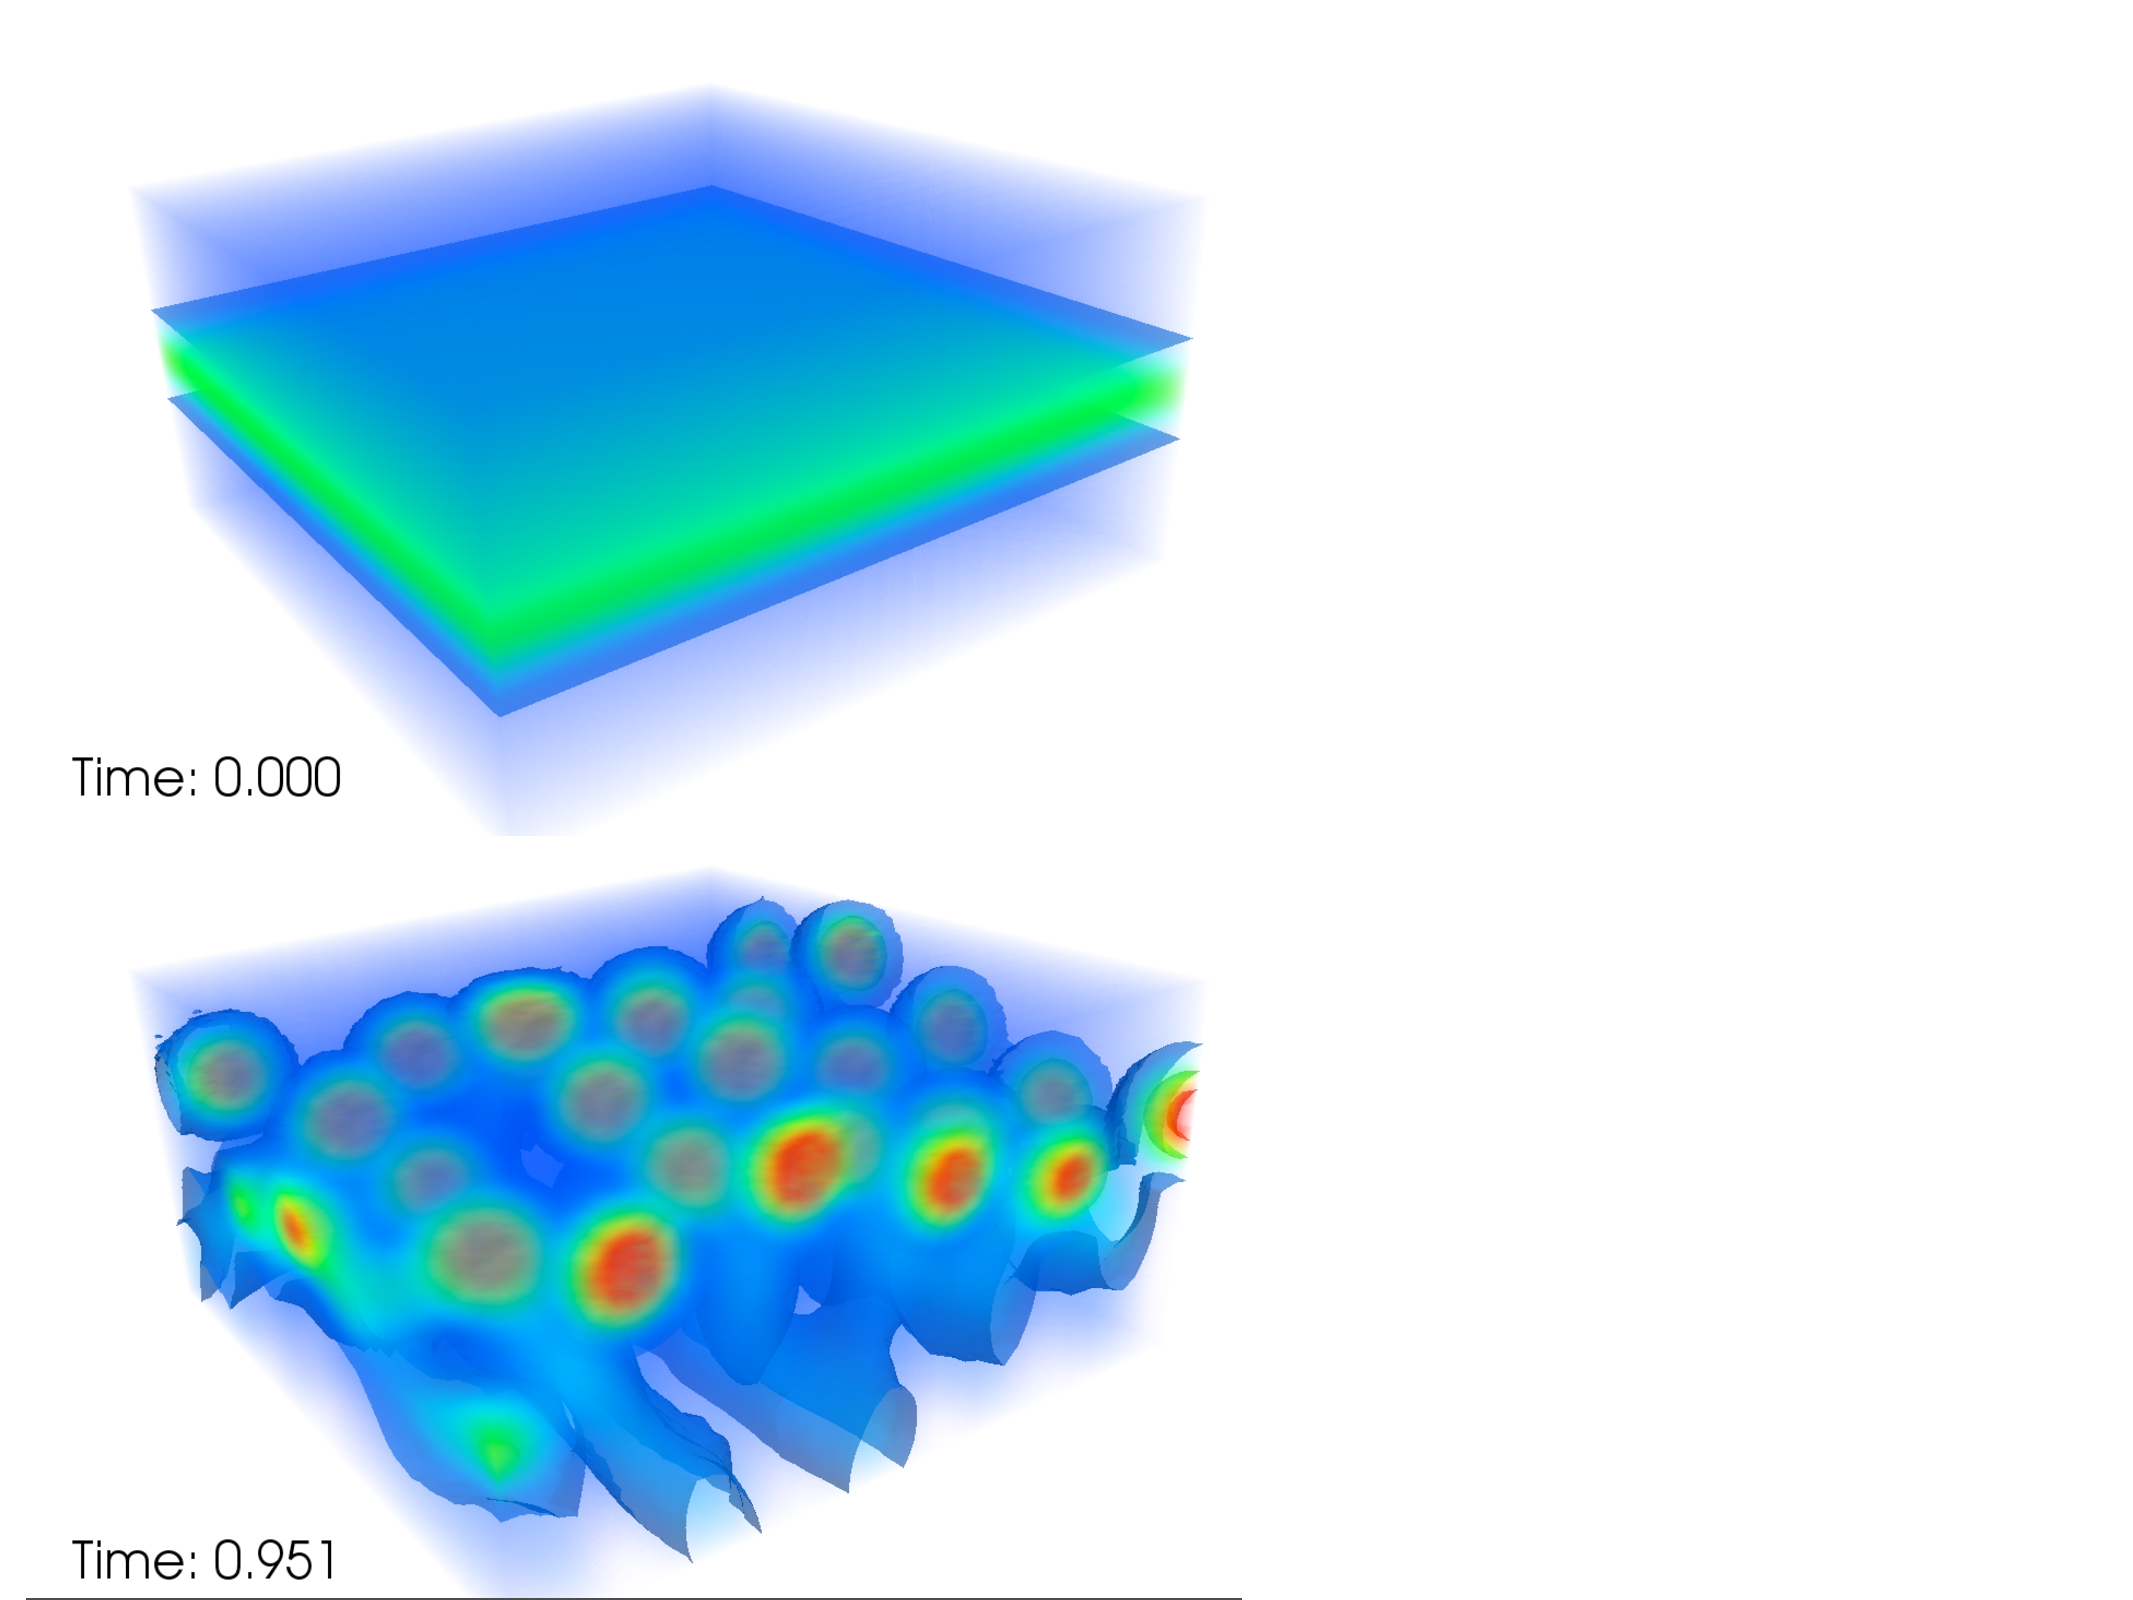
\includegraphics[width=.5\textwidth,clip=true]{figures/1dto3dwaves}
  \caption{Instability of 1D solitary wave to spherical 3D solitary waves.}
  \label{fig:1dto3dwaves}
\end{figure}

\begin{figure}[hb]
  \centering
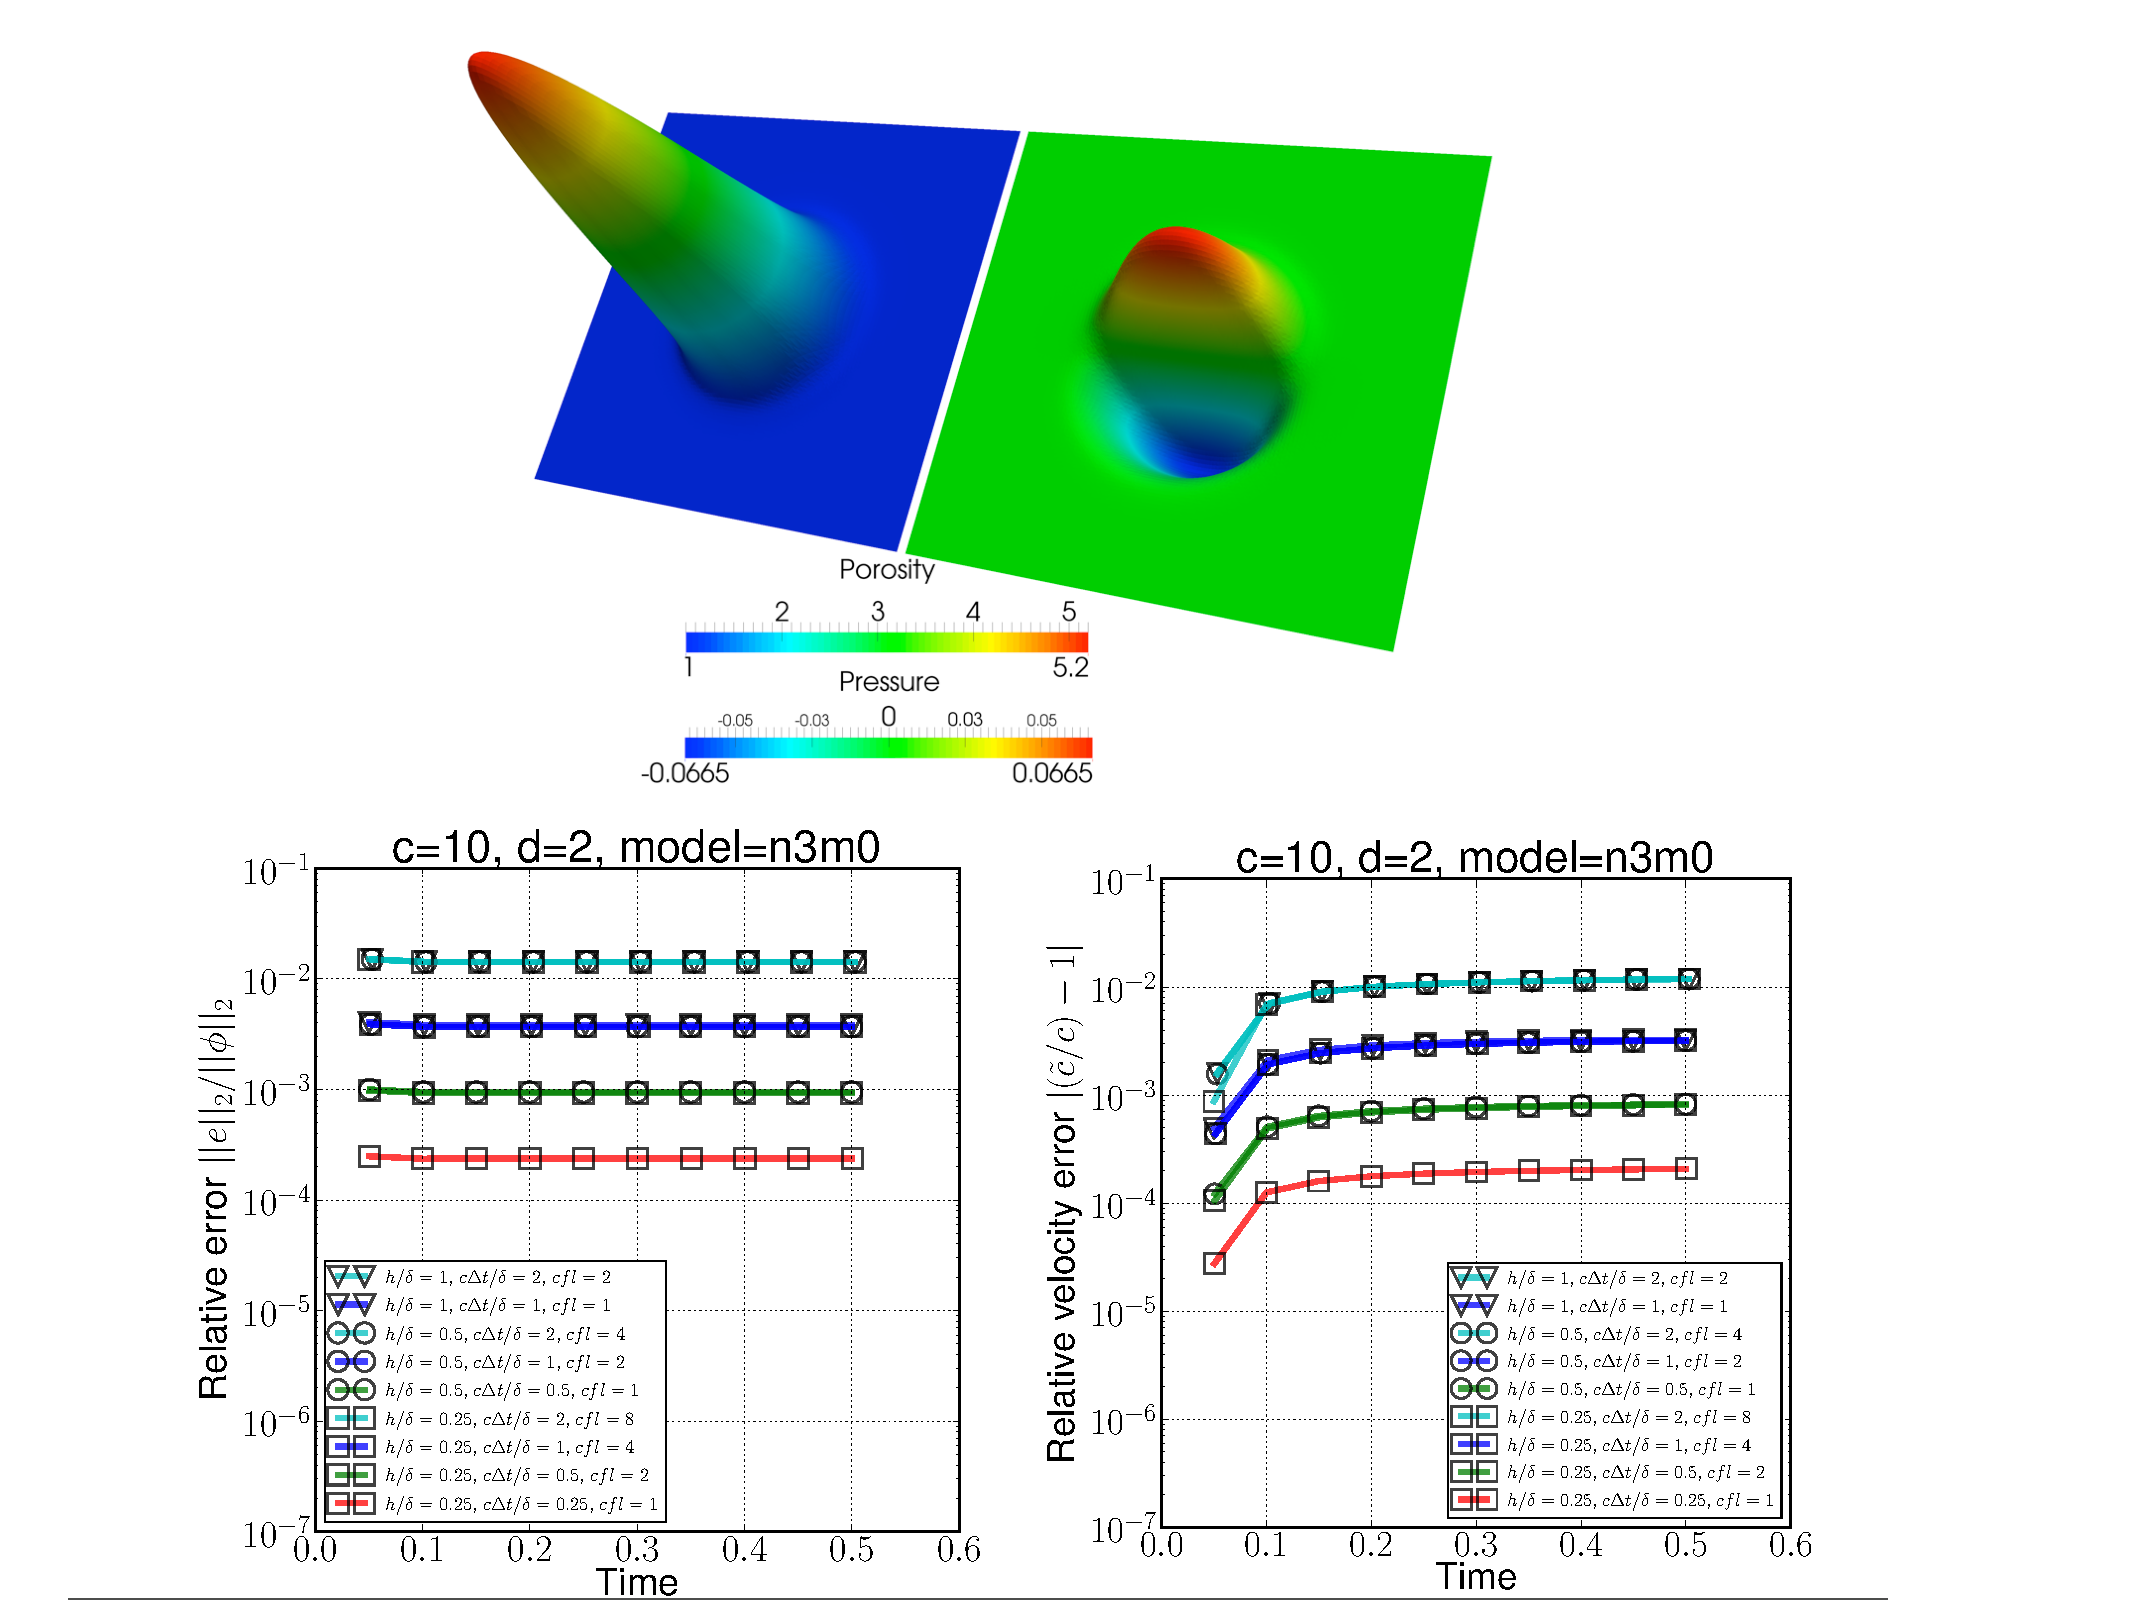
\includegraphics[width=.7\textwidth,clip=true]{figures/simpson_benchmark}
  \caption{Example magmatic solitary wave benchmarks from
    \cite{simpson_solitary_2011}. Top figure shows porosity and
    pressure fields for a 2D porosity wave with speed $c=10$,
    permeability exponent $n=3$, and bulk-viscosity exponent $m=0$.  These waves should propagate at constant porosity $c$
    without changing form and provides a fully non-linear benchmark
    problem. Lower figures show shape and velocity errors as a
    function of time. This benchmark solves the problem in a frame
    moving with the solitary waves using a semi-Lagrangian advection
    scheme in \TF{}. Additional results for other amplitude waves in
    2D and 3D, and other advection schemes are in Tables \ref{tab:simpson2d}--\ref{tab:simpson3d}.  }
  \label{fig:simpson_benchmarks}
\end{figure}

\begin{table*}[th!]
\caption{2D Solitary Wave Benchmarks
    \citep{simpson_solitary_2011}, phase and velocity errors as a
  function of grid-spacing and time step for waves with
  different parameters and background advection schemes, domain height
$h=64\delta$ compaction lengths.}
\begin{center}
  \begin{tabular}{ll}
\fbox{\begin{minipage}[c]{0.075\textwidth}\begin{sideways}\parbox{3.25cm}{\begin{center}$c=10,n=3,m=0$,\\semi-Lagrangian\end{center}}\end{sideways}\end{minipage}} 
&
\fbox{\begin{minipage}[c]{0.575\textwidth}\begin{tabular}{cccc}
     $N$ & $c\Delta t/\delta$  & $||\epsilon_{\phi}||$ & $\epsilon_{c}$  \\
32$\times$32 & 2.00 & 1.427786e-02 & 1.182138e-02  \\
32$\times$32 & 1.00 & 3.819159e-03 & 3.255477e-03  \\
32$\times$32 & 0.50 & 1.634865e-03 & 8.485232e-04  \\
32$\times$32 & 0.25 & 2.202831e-03 & 3.357135e-04  \\
64$\times$64 & 2.00 & 1.424202e-02 & 1.188175e-02  \\
64$\times$64 & 1.00 & 3.690917e-03 & 3.187174e-03  \\
64$\times$64 & 0.50 & 9.481209e-04 & 8.235713e-04  \\
64$\times$64 & 0.25 & 4.243532e-04 & 1.921914e-04  \\
128$\times$128 & 2.00 & 1.424087e-02 & 1.188190e-02  \\
128$\times$128 & 1.00 & 3.686779e-03 & 3.194658e-03  \\
128$\times$128 & 0.50 & 9.306871e-04 & 8.119311e-04  \\
128$\times$128 & 0.25 & 2.365556e-04 & 2.073026e-04  \\
\end{tabular}
\end{minipage}} \\
\\
\fbox{\begin{minipage}[c]{0.075\textwidth}\begin{sideways}\parbox{3.25cm}{\begin{center}$c=10,n=3,m=0$,\\CG\end{center}}\end{sideways}\end{minipage}} 
&
\fbox{\begin{minipage}[c]{0.575\textwidth}\begin{tabular}{cccc}
     $N$ & $c\Delta t/\delta$  & $||\epsilon_{\phi}||$ & $\epsilon_{c}$  \\
32$\times$32 & 2.00 & 1.427786e-02 & 1.182138e-02  \\
32$\times$32 & 1.00 & 3.819159e-03 & 3.255477e-03  \\
32$\times$32 & 0.50 & 1.634865e-03 & 8.485232e-04  \\
32$\times$32 & 0.25 & 2.202831e-03 & 3.357135e-04  \\
64$\times$64 & 2.00 & 1.424202e-02 & 1.188175e-02  \\
64$\times$64 & 1.00 & 3.690917e-03 & 3.187174e-03  \\
64$\times$64 & 0.50 & 9.481209e-04 & 8.235713e-04  \\
64$\times$64 & 0.25 & 4.243532e-04 & 1.921914e-04  \\
128$\times$128 & 2.00 & 1.424087e-02 & 1.188190e-02  \\
128$\times$128 & 1.00 & 3.686779e-03 & 3.194658e-03  \\
128$\times$128 & 0.50 & 9.306871e-04 & 8.119311e-04  \\
128$\times$128 & 0.25 & 2.365556e-04 & 2.073026e-04  \\
\end{tabular}
\end{minipage}} \\
\\
\fbox{\begin{minipage}[c]{0.075\textwidth}\begin{sideways}\parbox{3.25cm}{\begin{center}$c=4,n=2,m=1$,\\semi-Lagrangian\end{center}}\end{sideways}\end{minipage}} 
&
\fbox{\begin{minipage}[c]{0.575\textwidth}\begin{tabular}{cccc}
     $N$ & $c\Delta t/\delta$  & $||\epsilon_{\phi}||$ & $\epsilon_{c}$  \\
32$\times$32 & 2.00 & 1.427786e-02 & 1.182138e-02  \\
32$\times$32 & 1.00 & 3.819159e-03 & 3.255477e-03  \\
32$\times$32 & 0.50 & 1.634865e-03 & 8.485232e-04  \\
32$\times$32 & 0.25 & 2.202831e-03 & 3.357135e-04  \\
64$\times$64 & 2.00 & 1.424202e-02 & 1.188175e-02  \\
64$\times$64 & 1.00 & 3.690917e-03 & 3.187174e-03  \\
64$\times$64 & 0.50 & 9.481209e-04 & 8.235713e-04  \\
64$\times$64 & 0.25 & 4.243532e-04 & 1.921914e-04  \\
128$\times$128 & 2.00 & 1.424087e-02 & 1.188190e-02  \\
128$\times$128 & 1.00 & 3.686779e-03 & 3.194658e-03  \\
128$\times$128 & 0.50 & 9.306871e-04 & 8.119311e-04  \\
128$\times$128 & 0.25 & 2.365556e-04 & 2.073026e-04  \\
\end{tabular}
\end{minipage}} \\
\\
\fbox{\begin{minipage}[c]{0.075\textwidth}\begin{sideways}\parbox{3.25cm}{\begin{center}$c=4,n=2,m=1$,\\CG\end{center}}\end{sideways}\end{minipage}} 
&
\fbox{\begin{minipage}[c]{0.575\textwidth}\begin{tabular}{cccc}
     $N$ & $c\Delta t/\delta$  & $||\epsilon_{\phi}||$ & $\epsilon_{c}$  \\
32$\times$32 & 2.00 & 1.427786e-02 & 1.182138e-02  \\
32$\times$32 & 1.00 & 3.819159e-03 & 3.255477e-03  \\
32$\times$32 & 0.50 & 1.634865e-03 & 8.485232e-04  \\
32$\times$32 & 0.25 & 2.202831e-03 & 3.357135e-04  \\
64$\times$64 & 2.00 & 1.424202e-02 & 1.188175e-02  \\
64$\times$64 & 1.00 & 3.690917e-03 & 3.187174e-03  \\
64$\times$64 & 0.50 & 9.481209e-04 & 8.235713e-04  \\
64$\times$64 & 0.25 & 4.243532e-04 & 1.921914e-04  \\
128$\times$128 & 2.00 & 1.424087e-02 & 1.188190e-02  \\
128$\times$128 & 1.00 & 3.686779e-03 & 3.194658e-03  \\
128$\times$128 & 0.50 & 9.306871e-04 & 8.119311e-04  \\
128$\times$128 & 0.25 & 2.365556e-04 & 2.073026e-04  \\
\end{tabular}
\end{minipage}}
  \end{tabular}
\end{center}
\label{tab:simpson2d}
\end{table*}

\begin{table*}[th!]
\caption{3D Solitary Wave Benchmarks
    \citep{simpson_solitary_2011}, phase and velocity errors as a
  function of grid-spacing and time step, CG advection, $c=5$, $n=3$,
  $m=0$ waves}
\begin{center}
  \begin{tabular}{ll}
\fbox{\begin{minipage}[c]{0.075\textwidth}\begin{sideways}\parbox{3.25cm}{\begin{center}$h/\delta=64$\end{center}}\end{sideways}\end{minipage}} 
&
\fbox{\begin{minipage}[c]{0.575\textwidth}\begin{tabular}{cccc}
     $N$ & $c\Delta t/\delta$  & $||\epsilon_{\phi}||$ & $\epsilon_{c}$  \\
32$\times$32 & 2.00 & 1.427786e-02 & 1.182138e-02  \\
32$\times$32 & 1.00 & 3.819159e-03 & 3.255477e-03  \\
32$\times$32 & 0.50 & 1.634865e-03 & 8.485232e-04  \\
32$\times$32 & 0.25 & 2.202831e-03 & 3.357135e-04  \\
64$\times$64 & 2.00 & 1.424202e-02 & 1.188175e-02  \\
64$\times$64 & 1.00 & 3.690917e-03 & 3.187174e-03  \\
64$\times$64 & 0.50 & 9.481209e-04 & 8.235713e-04  \\
64$\times$64 & 0.25 & 4.243532e-04 & 1.921914e-04  \\
128$\times$128 & 2.00 & 1.424087e-02 & 1.188190e-02  \\
128$\times$128 & 1.00 & 3.686779e-03 & 3.194658e-03  \\
128$\times$128 & 0.50 & 9.306871e-04 & 8.119311e-04  \\
128$\times$128 & 0.25 & 2.365556e-04 & 2.073026e-04  \\
\end{tabular}
\end{minipage}} \\
\\
\fbox{\begin{minipage}[c]{0.075\textwidth}\begin{sideways}\parbox{3.25cm}{\begin{center}$h/\delta=32$\\(higher resolution)\end{center}}\end{sideways}\end{minipage}} 
&
\fbox{\begin{minipage}[c]{0.575\textwidth}\begin{tabular}{cccc}
     $N$ & $c\Delta t/\delta$  & $||\epsilon_{\phi}||$ & $\epsilon_{c}$  \\
32$\times$32 & 2.00 & 1.427786e-02 & 1.182138e-02  \\
32$\times$32 & 1.00 & 3.819159e-03 & 3.255477e-03  \\
32$\times$32 & 0.50 & 1.634865e-03 & 8.485232e-04  \\
32$\times$32 & 0.25 & 2.202831e-03 & 3.357135e-04  \\
64$\times$64 & 2.00 & 1.424202e-02 & 1.188175e-02  \\
64$\times$64 & 1.00 & 3.690917e-03 & 3.187174e-03  \\
64$\times$64 & 0.50 & 9.481209e-04 & 8.235713e-04  \\
64$\times$64 & 0.25 & 4.243532e-04 & 1.921914e-04  \\
128$\times$128 & 2.00 & 1.424087e-02 & 1.188190e-02  \\
128$\times$128 & 1.00 & 3.686779e-03 & 3.194658e-03  \\
128$\times$128 & 0.50 & 9.306871e-04 & 8.119311e-04  \\
128$\times$128 & 0.25 & 2.365556e-04 & 2.073026e-04  \\
\end{tabular}
\end{minipage}}
  \end{tabular}
\end{center}
\label{tab:simpson3d}
\end{table*}

